\section{Figures of merit per channel}\label{sec:17.5}

The heavy-mediator plateau of single-phonon emission is 1101 events per kilogram and year in germanium and 654 in silicon at $\sigma_p = 10^{-40}\,\mathrm{cm^2}$ (\cref{sec:11.1}). The ratio, 1.68, is the ratio of two sound speeds, and once the elastic tensors are known no phonon calculation is needed to obtain it. A number of this kind, a property of the material alone that the rate or the reach of one channel is proportional to, is what a comparison of targets needs. Such numbers exist for most channels of \cref{chap:10,chap:11,chap:12}, but each holds over a window of masses, and outside it the ratio of two rates is not the ratio of the two numbers. We will derive one such number per channel, with its window and inputs.

\subsection{Rate and reach figures of merit}\label{sec:17.5-def}

A figure of merit is either a reach number or a rate number. A \emph{reach figure of merit} is the lightest mass a channel can see, set by kinematics and one material energy or speed: the gap floor $2\Eg/v_{\mathrm{max}}^2$ of electronic excitations (\cref{eq:1.3-mmin}), the acoustic edge \cref{eq:11.1-edge}, the polar edge $2\omega_{\mathrm{L}}/v_{\mathrm{max}}^2$. These are exact statements about where a rate starts, and they rank materials without a window. A \emph{rate figure of merit} $F_A$ of material $A$ is a number that makes the rate per unit target mass factorize at fixed dark-matter parameters, $\mathcal{R}_A(\mchi) = G(\mchi)\,F_A$, with $G$ the same for every material. No real rate factorizes exactly, and the useful statement is about pairs. For two materials $A$ and $B$ we write
\begin{equation}
  \frac{\mathcal{R}_A(\mchi)}{\mathcal{R}_B(\mchi)} = \frac{F_A}{F_B}\,\bigl[1 + \delta_{AB}(\mchi)\bigr] ,
  \qquad
  W_{AB} = \bigl\{\mchi : |\delta_{AB}(\mchi)| < 0.1\bigr\} ,
  \label{eq:17.5-window}
\end{equation}
and call the contiguous range $W_{AB}$ the \emph{pairwise window} of the figure of merit, the masses at which the ratio of the two figures of merit gives the ratio of the rates to \SI{10}{\percent}. The tolerance is a convention, chosen to match the accuracy of most inputs. A window belongs to a pair, not to a material, because the corrections $\delta$ of two materials partly cancel when their properties are close and add when they are not. Several materials have a common window only if every pair among them has one, and \cref{sec:17.5-phonon} shows that this fails for sound speeds. \Cref{tab:17-fom} collects the figures of merit of every channel with their windows and the provenance of their inputs.

\begin{table}[tbp]
\centering
\caption{Figures of merit per channel, with the masses at which they rank two materials and the provenance of their inputs. Rates per unit target mass; $\omega_{\mathrm{th}} = \SI{1}{meV}$ for the phonon channels; standard halo of \cref{sec:1.2}. ``Pairwise'' refers to the window \cref{eq:17.5-window}. The absorption figures of merit are exact at each mass, since absorption fixes both $q$ and $\omega$.}
\label{tab:17-fom}
\footnotesize
\begin{tabular}{>{\raggedright\arraybackslash}p{0.13\linewidth}>{\raggedright\arraybackslash}p{0.19\linewidth}>{\raggedright\arraybackslash}p{0.27\linewidth}>{\raggedright\arraybackslash}p{0.16\linewidth}>{\raggedright\arraybackslash}p{0.09\linewidth}}
\toprule
Channel & Figure of merit & Where it ranks & Inputs & Silicon \\
\midrule
Electronic, reach & $2\Eg/v_{\mathrm{max}}^2$ & exact & $\Eg(T)$, measured & \SI{0.333}{MeV} \\
Electronic, rate & $L(q,\omega)$ in the window; ceiling $\propto Z_{\mathrm{val}}/A_{\mathrm{cell}}$ & no scalar ranks rates; ceiling with $\omega_p^{\mathrm{val}}$ for $qv_{\mathrm{max}} < \omega_{\mathrm{core}}$ (\cref{eq:17.5-partial}) & $L$ computed; $\nd_{\mathrm{val}}$, $\omega_p^{\mathrm{val}}$ measured & 0.142 \\
Acoustic, reach & $m_{\mathrm{min}}^{\mathrm{ac}}$ at $c_{\mathrm{LA,max}}$, \cref{eq:11.1-edge} & exact & $C_{ij}$, $\rho_T$ & \SI{6.1}{keV} \\
Acoustic, heavy mediator & $1/c_{\mathrm{NR1}}$, \cref{eq:17.5-cNR1} & pairwise: from about 4 edges of the softer crystal to the smaller $q_{\mathrm{BZ}}/2v_{\mathrm{max}}$; empty if speeds differ by $\gtrsim\SI{13.5}{km/s}$ & $C_{ij}$ measured or computed & 8.956\,km/s \\
Acoustic, light mediator & none (target independent) & equal rates above 44 times the higher edge & edge only & -- \\
Polar, rate & $\mathcal{I}_{\mathrm{pol}}/\rho_T$ with $\bar\omega_{\mathrm{pol}}$ & with $K_\eta(\bar\omega_{\mathrm{pol}},\mchi)$ at each mass; $\mathcal{I}_{\mathrm{pol}}/\rho_T$ alone only where the $K_\eta$ agree (LiF/GaAs above \SI{52}{MeV}) & $\varepsilon_\infty$, $\varepsilon_0$, $\omega_{\mathrm{T}\nu}$, $\omega_{\mathrm{L}\nu}$ measured, or $Z^*$ computed & -- \\
Polar, reach & $2\omega_{\mathrm{L}\nu}/v_{\mathrm{max}}^2$, lowest weighted branch & exact & $\omega_{\mathrm{L}\nu}$, measured & -- \\
Migdal & $F_{\mathrm{Mig}}$; pole limit \cref{eq:17.5-pole} & impulse regime (Si above \SI{17.5}{MeV}); ranking open & $L(p,\omega)$, $Z_{\mathrm{ion}}(p)$ computed & pole: 0.570, \SI{16.6}{eV} \\
Absorption & $L(0,m_\phi)/\rho_T$, $m_\phi\sigma_1/\rho_T$, scalar response per mass (\cref{sec:17.2}) & exact at each mass & optical data or computed & \cref{sec:17.2} \\
\bottomrule
\end{tabular}
\end{table}

\subsection{Gap floor and valence f-sum}\label{sec:17.5-electronic}

An electronic excitation needs at least $\Eg$, and the dark matter can deposit at most $\frac12\mchi v_{\mathrm{max}}^2$ (\cref{eq:1.3-omegamax}). The floor $2\Eg/v_{\mathrm{max}}^2$ is \SI{0.333}{MeV} for silicon with its physical gap of \SI{1.17}{eV}, \SI{0.212}{MeV} for germanium (\SI{0.744}{eV}) and \SI{0.433}{MeV} for GaAs (\SI{1.52}{eV}); with the step-model gap of \SI{1.11}{eV} that accompanies the silicon tables (\cref{sec:10.10}), it is \SI{0.316}{MeV}. Near the floor the rate is set by the spectrum within a few phonon energies of the edge. The gap is a measured input, and it must be the gap at the operating temperature of the detector, since the floor moves by the same fraction as the gap.

A rate figure of merit is harder. The electron-recoil rate weights the loss function over the window $\omega \le qv_{\mathrm{max}}$ by the halo factor. \Cref{we:10-fsum} showed that silicon puts a tiny part of its $f$-sum where a \SI{1}{MeV} particle can reach it: the computed rate is $4\times10^6$ times below the all-electron ceiling. Since the weight of the loss function inside the window varies between materials by orders of magnitude, no single number ranks electron-recoil rates; the loss function in the window is the figure of merit itself. What a single number can give is the ceiling. For it to be useful, the ceiling must count the electrons that absorb in the window and no others, and that needs a partial $f$-sum.

Split the dielectric function of an insulator with clamped nuclei into the contributions of the valence electrons and of the core,
\begin{equation*}
  \varepsilon(\omega) = \varepsilon_{\mathrm{val}}(\omega) + \varepsilon_{\mathrm{core}}(\omega) - 1 ,
\end{equation*}
each of them one plus the polarization of its group, at $q \to 0$. Three conditions make the valence part separable. (i) The two groups add, so that each obeys its own $f$-sum, $\int_0^\infty\dd\omega\,\omega\,\Imag\varepsilon_{\mathrm{val}} = (\pi/2)(\omega_p^{\mathrm{val}})^2$ with $(\omega_p^{\mathrm{val}})^2 = e^2\nd_{\mathrm{val}}/m_e$; this neglects the transfer of oscillator strength between shells that the Pauli principle causes (\cref{we:4-sifsum}). (ii) The valence absorption ends below the first core edge $\omega_{\mathrm{core}}$, and the core does not absorb below it. (iii) Over the valence spectrum the core part is real and equal to its static value, $\varepsilon_{\mathrm{core}}(\omega) \simeq \varepsilon_{\mathrm{core}}(0)$, which holds to order $\omega^2/\omega_{\mathrm{core}}^2$. By the Kramers--Kronig relation at $\omega = 0$ (\cref{eq:C.5-KKeps}),
\begin{equation*}
  \varepsilon_{\mathrm{core}}(0) - 1 = \frac{2}{\pi}\int_{\omega_{\mathrm{core}}}^\infty\dd\omega\,\frac{\Imag\varepsilon_{\mathrm{core}}(\omega)}{\omega} .
\end{equation*}
Below $\omega_{\mathrm{core}}$ we then have $\varepsilon = \varepsilon_{\mathrm{core}}(0) + \varepsilon_{\mathrm{val}} - 1$. Consider the model function $\varepsilon_{\mathrm{m}}(\omega) = \varepsilon_{\mathrm{core}}(0) + \varepsilon_{\mathrm{val}}(\omega) - 1$ at all frequencies, which equals $\varepsilon$ below the core edge to order $\omega^2/\omega_{\mathrm{core}}^2$. Above the valence spectrum $\varepsilon_{\mathrm{val}} - 1 \to -(\omega_p^{\mathrm{val}})^2/\omega^2$, so the function $g(\omega) = \varepsilon_{\mathrm{m}}^{-1}(\omega) - 1/\varepsilon_{\mathrm{core}}(0)$ falls as $(\omega_p^{\mathrm{val}})^2/[\varepsilon_{\mathrm{core}}(0)^2\omega^2]$. It is analytic in the upper half plane, being the inverse of a causal response with a constant subtracted, and the argument that turns the large-frequency tail of $\varepsilon^{-1}$ into the $f$-sum of the loss function (\cref{eq:4.4-fsumL}, \cref{app:C.5}) applies to it. For the true $\varepsilon$ the same tail is an intermediate asymptote, valid between the valence spectrum and the core edge, since at $\omega \to \infty$ the true $g$ tends to $1 - 1/\varepsilon_{\mathrm{core}}(0)$. Since $\Imag[-g] = L$ below $\omega_{\mathrm{core}}$, the loss function collected up to a cutoff $\omega_c$ between the valence spectrum and the core edge is
\begin{keyresult}[Partial (valence) f-sum of the loss function]
\begin{equation}
  \int_0^{\omega_c}\dd\omega\;\omega\,L(\omega) = \frac{\pi}{2}\,\frac{(\omega_p^{\mathrm{val}})^2}{\varepsilon_{\mathrm{core}}(0)^2} \simeq \frac{\pi}{2}\,(\omega_p^{\mathrm{val}})^2 ,
  \label{eq:17.5-partial}
\end{equation}
with $\omega_p^{\mathrm{val}}$ the plasma frequency of the valence electrons alone.
\end{keyresult}
\noindent The core screens the valence plasmon and lowers its weight by $\varepsilon_{\mathrm{core}}(0)^{-2}$. The absorption $\Imag\varepsilon$ collected over the same range carries no such factor, because $\varepsilon$ adds where $\varepsilon^{-1}$ does not. For silicon, $\nd_{\mathrm{val}} = \SI{2.00e23}{cm^{-3}}$ gives $\omega_p^{\mathrm{val}} = \SI{16.6}{eV}$ (\cref{we:4-siplasmon}), the measured plasmon energy, $16.6 \pm \SI{0.1}{eV}$ by electron energy loss~\cite[Table~I]{ramanathan2020ionization}. The core term follows from the photoabsorption above the L edge at \SI{99.8}{eV}: $\varepsilon_{\mathrm{core}}(0) - 1 = 0.0154$, so the core lowers the valence weight of $L$ by the factor $0.970$. A valence-only calculation, such as the tables of \cref{sec:10.2}, has no core and satisfies \cref{eq:17.5-partial} with $\varepsilon_{\mathrm{core}} = 1$; this is why \SI{16.6}{eV} is the right normalization of those tables (\cref{we:12-fsum}).

\begin{limitbox}[Partial f-sum of the valence electrons][lim:17.5a]
Below the first core edge the valence electrons carry the $f$-sum of the loss function $\int_0^{\omega_c}\omega L\,\dd\omega = (\pi/2)(\omega_p^{\mathrm{val}})^2$, with $\omega_p^{\mathrm{val}} = \SI{16.6}{eV}$ for silicon, the measured plasmon energy~\cite[Table~I]{ramanathan2020ionization}.
\par\smallskip
{\centering
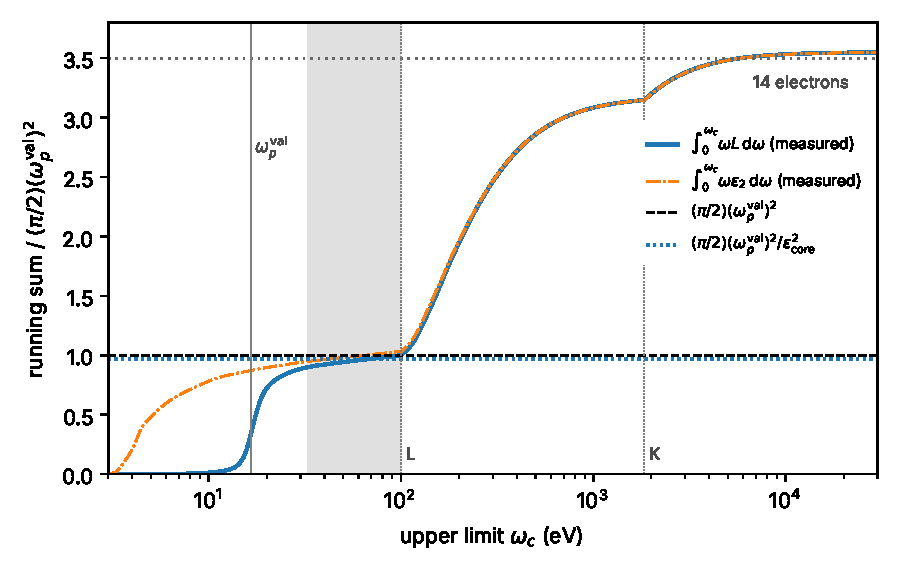
\includegraphics[width=\linewidth]{figures/ch17/limit17_5a.pdf}
\captionof{figure}{Running $f$-sums of silicon at $q \to 0$, $\int_0^{\omega_c}\omega L\,\dd\omega$ (solid) and $\int_0^{\omega_c}\omega\varepsilon_2\,\dd\omega$ (dash-dotted), in units of $(\pi/2)(\omega_p^{\mathrm{val}})^2 = \SI{433}{eV^2}$, against the upper limit $\omega_c$. Data: the measured optical constants of Franta and coworkers at \SI{300}{K} below \SI{35}{eV}~\cite{franta2017temperature} and the photoabsorption tables of Henke and coworkers above, with $\varepsilon = 1 - (\omega_a^2/\omega^2)(f_1 - \ii f_2)$, $\omega_a^2 = e^2\nd_{\mathrm{at}}/m_e$~\cite{henke1993xray}; moving the join to 30 or \SI{40}{eV} changes the $L$-sum below the L edge by \SI{0.8}{\percent}. Dashed: \cref{eq:17.5-partial} with $\varepsilon_{\mathrm{core}} = 1$; dotted: with the core term, 0.970. Vertical lines: $\omega_p^{\mathrm{val}}$ and the L and K edges at 99.8 and \SI{1839}{eV}; the dotted horizontal line at 3.5 is the sum of all 14 electrons per atom. Gray: $\omega_c$ from \SI{32.7}{eV} to the L edge, where the $L$-sum lies within \SI{10}{\percent} of the formula; just below the edge it is 1.000.}\label{fig:17-limit-a}
\par}
\smallskip
Below about $2\omega_p^{\mathrm{val}}$ the plasmon is not yet collected, and above the L edge the core electrons add their own sum, which rises toward 3.5 times the valence value.
\end{limitbox}

Just below the edge the measured $L$-sum is 1.000 of $(\pi/2)(\omega_p^{\mathrm{val}})^2$ and the $\varepsilon_2$-sum 1.032. The two corrections to \cref{eq:17.5-partial} are of similar size and opposite sign. The core screening lowers the $L$-sum by \SI{3}{\percent}, and the valence region holds \SI{3}{\percent} more absorption than four electrons, the strength moved up from the blocked core transitions. The data fix each of them to \SI{1.4}{\percent}, the amount by which the two sets together overshoot the all-electron sum of 14. The approach to the plateau is slow, because the plasmon at \SI{16.4}{eV} is broad: the $L$-sum reaches 0.9 at \SI{32.7}{eV}.

The partial sum turns the valence plasma frequency into a usable ceiling. \Cref{we:10-fsum} found that $\omega_p^{\mathrm{val}}$ in place of the all-electron \SI{31.1}{eV} does not give a bound, since the core electrons hold the rest of the $f$-sum. When the window lies entirely below the core edge, however, the energy integral of the bound runs over the valence spectrum alone, and by \cref{eq:17.5-partial} its weight is $(\pi/2)(\omega_p^{\mathrm{val}})^2$ to the few-percent accuracy of the two corrections; at finite $q$ the condition is $qv_{\mathrm{max}} < \omega_{\mathrm{core}}$. This is not a theorem, since the corrections need not stay small at finite $q$, but it lowers the ceiling of silicon by $(31.1/16.6)^2 = 3.5$ for every mass whose largest deposit, $\frac12\mchi v_{\mathrm{max}}^2$, lies below the L edge, $\mchi < \SI{28.4}{MeV}$. Per unit target mass the ceiling is proportional to $(\omega_p^{\mathrm{val}})^2/\rho_T = e^2Z_{\mathrm{val}}/(m_em_uA_{\mathrm{cell}})$, with $Z_{\mathrm{val}}$ valence electrons in a cell of $A_{\mathrm{cell}}$ mass units: the number of valence electrons per nucleon, 0.142 for silicon, 0.055 for germanium, 0.333 for diamond and 0.308 for LiF. This orders the ceilings, not the rates, which differ from them by the factor $10^{6}$ of \cref{we:10-fsum}.

\subsection{Acoustic edge and effective sound speed}\label{sec:17.5-phonon}

The one-phonon rate of \cref{eq:11.1-rate} has three figures of merit, one for each limit of the mediator and one for the edge. The reach figure of merit is the acoustic edge \cref{eq:11.1-edge}, evaluated at the fastest longitudinal speed $c_{\mathrm{LA,max}}$: \SI{6.1}{keV} for silicon, \SI{10.2}{keV} for germanium and \SI{3.1}{keV} for diamond at $\omega_{\mathrm{th}} = \SI{1}{meV}$. It is exact kinematics and ranks without a window. A stiff crystal reaches lower masses.

For a light mediator there is no rate figure of merit. The rate per unit mass tends to the target-independent value \cref{eq:11.1-light}, and the material enters through the correction factor $1 - (1 + \kappa_\eta)\,m_{\mathrm{min}}^{\mathrm{ac}}/\mchi$ alone, with the constant $\kappa_\eta$ of \cref{eq:11.1-correction}. Two materials have equal rates within \SI{10}{\percent} above 44 times the higher of their two edges (\cref{lim:11.1b}), and below that the edge, a reach number, decides.

For a heavy mediator, \cref{eq:11.1-heavy} gives a plateau inversely proportional to the polarization-weighted mean of the inverse sound speeds. Its inverse is an effective sound speed of the one-phonon nuclear rate,
\begin{equation}
  c_{\mathrm{NR1}} = \Bigl\langle\sum_\nu\frac{(\hat{\vect{q}}\cdot\hat{\vect{e}}_\nu)^2}{c_\nu(\hat{\vect{q}})}\Bigr\rangle_{\hat{\vect{q}}}^{-1} ,
  \qquad
  \mathcal{R} = \frac{2\rho_\chi\,\sigma_p\,I_0}{m_u^2\,c_{\mathrm{NR1}}} ,
  \label{eq:17.5-cNR1}
\end{equation}
so that the figure of merit is $1/c_{\mathrm{NR1}}$. It is \SI{8.956}{km/s} for silicon, \SI{5.321}{km/s} for germanium and \SI{18.16}{km/s} for diamond, within one percent of the sphere-averaged longitudinal speeds (\cref{lim:11.1c}) for these weakly anisotropic crystals. The speeds and polarizations come from the Christoffel problem of the elastic tensor (\cref{eq:C.18-christoffel}). The tensor is measured from the speed of ultrasound or from light scattered by thermal sound waves, or computed by density-functional theory from finite strains or from perturbation theory with strain as the perturbation (\cref{app:E.4}); \cref{app:E.17} specifies the elastic constants needed for the candidate targets. The two figures of merit pull in opposite directions: a soft lattice gives a large heavy-mediator rate and a high edge.

\Cref{eq:17.5-cNR1} drops two things, and each sets one end of the window. At low mass the lower cut $u_- = \omega_{\mathrm{th}}/(2\mchi c_\nu)$ of the integral $\int u^2\eta(c_\nu + u)\,\dd u$ removes the slowest part of the halo integral. Since $u_- = (v_{\mathrm{max}} - c_\nu)\,m_{\mathrm{min}}^{\mathrm{ac}}/\mchi$, it is a function of the mass in units of the edge, and it closes the window from below at a few times the edge of the softer crystal. At high mass the momentum transfers reach the zone scale, \cref{eq:11.1-Sac} stops holding, and the window ends at $m_{\mathrm{hi}} = q_{\mathrm{BZ}}/2v_{\mathrm{max}}$ of the crystal with the smaller zone, \SI{0.42}{MeV} for silicon (\cref{sec:11.1}). Between the two ends the window would be complete if the plateau were exact. It is not, and the reason is the shift of the halo integral by the sound speed.

Far above the edge, the integral of one branch and direction is $8\mchi^3\int_0^{v_{\mathrm{max}} - c_\nu}\dd u\,u^2\eta(c_\nu + u)$. With $v = c_\nu + u$ it becomes $8\mchi^3\int_{c_\nu}^{v_{\mathrm{max}}}\dd v\,(v - c_\nu)^2\eta(v)$, and expanding the square,
\begin{equation*}
  \int_{c_\nu}^{v_{\mathrm{max}}}\dd v\,(v - c_\nu)^2\eta(v) = I_0 - 2c_\nu I_1 + c_\nu^2 + O(c_\nu^3) ,
  \qquad
  I_1 = \int_0^{v_{\mathrm{max}}}\dd v\,v\,\eta(v) ,
\end{equation*}
where $I_0$ is the plateau integral of \cref{sec:11.1}. The coefficient of $c_\nu^2$ is $\int_0^\infty\eta\,\dd v = 1$, the normalization of the velocity distribution, since $\eta$ is its integral of $f_\chi/v$ above $\vmin$. The integral from $0$ to $c_\nu$ is of third order. Each branch and direction carries the weight $(\hat{\vect{q}}\cdot\hat{\vect{e}}_\nu)^2/c_\nu$, so the term $-2c_\nu I_1$ contributes $-2I_1\langle\sum_\nu(\hat{\vect{q}}\cdot\hat{\vect{e}}_\nu)^2\rangle = -2I_1$ by completeness, independent of the crystal. The rate in units of the plateau is
\begin{equation}
  \frac{\mathcal{R}\,c_{\mathrm{NR1}}\,m_u^2}{2\rho_\chi\sigma_pI_0} = 1 - \frac{2I_1}{I_0}\,c_{\mathrm{NR1}} + O(c^2) ,
  \qquad
  \frac{2I_1}{I_0} = \frac{5.88}{v_{\mathrm{max}}} = \frac{1}{\SI{135}{km/s}} ,
  \label{eq:17.5-shift}
\end{equation}
for the standard halo of \cref{sec:1.2}, with $\eta$ evaluated at $\vmin = c_\nu + q/2\mchi$ as in \cref{eq:11.1-rate}. For silicon the bracket is 0.934 at first order and 0.935 at second, against the largest computed ratio 0.936; for diamond 0.866 and 0.872, against 0.874. This is why the plateau of \cref{sec:11.1} is never reached: the halo is not flat at the large speeds that a heavy mediator favors.

The shift is linear in the sound speed and does not cancel between materials. For two crystals in the middle of their window,
\begin{equation*}
  \frac{\mathcal{R}_A\,c_{\mathrm{NR1},A}}{\mathcal{R}_B\,c_{\mathrm{NR1},B}} \simeq 1 - \frac{c_{\mathrm{NR1},A} - c_{\mathrm{NR1},B}}{\SI{135}{km/s}} .
\end{equation*}
Roughly, the inverse speeds rank two crystals to \SI{10}{\percent} as long as their effective speeds differ by less than \SI{13.5}{km/s}, which diamond and germanium, \SI{12.8}{km/s} apart, barely meet. The deviations of several crystals from a common reference add linearly in their speeds, and two crystals that both agree with silicon to \SI{10}{\percent} can disagree with each other by up to twice that. \Cref{fig:17-window} shows the ratio for five pairs. Germanium against silicon enters the band at \SI{43}{keV} and settles at 1.027; diamond against silicon enters at \SI{25}{keV} and settles at 0.933; CsI, a soft cubic crystal discussed below, enters at \SI{97}{keV} and reaches 1.045 at its zone cap. Diamond against CsI, however, is inside the band from 87 to \SI{227}{keV} alone and leaves it below the cap, where both still agree with silicon. A window ``against silicon'' does not give the ranking of the materials among themselves, and every pair needs its own.

\begin{figure}[tbp]
  \centering
  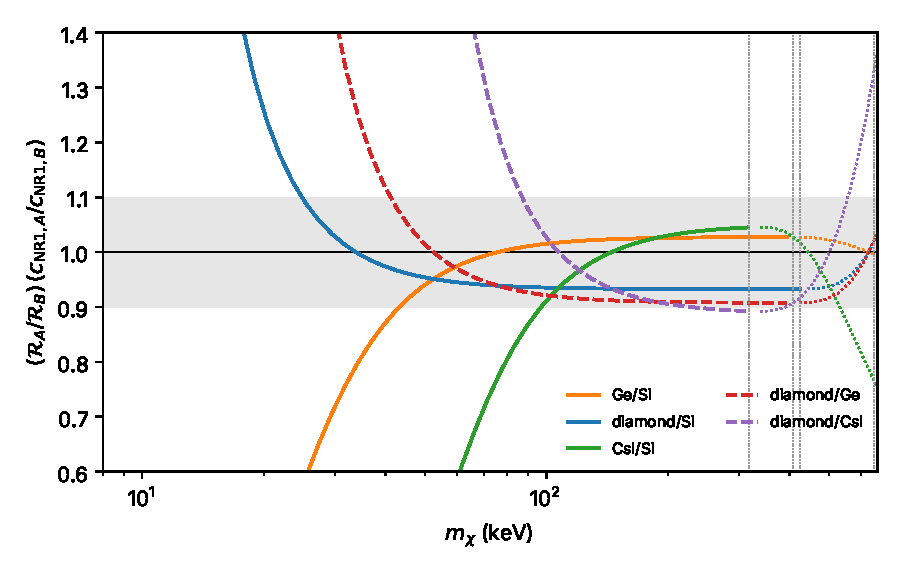
\includegraphics[width=0.85\linewidth]{figures/ch17/fig17_window.pdf}
  \caption{Heavy-mediator one-phonon rates of two crystals divided by the ratio of their figures of merit, $(\mathcal{R}_A/\mathcal{R}_B)(c_{\mathrm{NR1},A}/c_{\mathrm{NR1},B})$, against the dark-matter mass, from \cref{eq:11.1-rate} with all branches and directions, $q \le q_{\mathrm{BZ}}$, $\omega_{\mathrm{th}} = \SI{1}{meV}$, the orientation average and the standard halo of \cref{sec:1.2}. Elastic tensors: measured room-temperature values for Si, Ge and diamond (\cref{we:11-cbar}); CsI at \SI{4.2}{K}~\cite{vallin1964elastic} with the room-temperature density \SI{4.529}{g.cm^{-3}}. Gray: the \SI{10}{\percent} band of the pairwise window \cref{eq:17.5-window}. Each curve is solid up to the smaller $q_{\mathrm{BZ}}/2v_{\mathrm{max}}$ of its pair (vertical dotted lines: 0.32, 0.41, 0.42 and \SI{0.65}{MeV} for CsI, Ge, Si and diamond) and dotted above. At high mass the curves settle at $1 - (c_{\mathrm{NR1},A} - c_{\mathrm{NR1},B})/(\SI{135}{km/s})$, \cref{eq:17.5-shift}.}
  \label{fig:17-window}
\end{figure}

\begin{workedexample}{The pairwise window of diamond against silicon}\label{we:17-window}
Diamond has $c_{\mathrm{NR1}} = \SI{18.16}{km/s}$ and silicon \SI{8.956}{km/s}, so the figure of merit predicts a heavy-mediator rate ratio of $8.956/18.16 = 0.493$: the plateaus of \cref{eq:17.5-cNR1} are 322.6 and 654.0 events per kilogram and year at $\sigma_p = 10^{-40}\,\mathrm{cm^2}$ and $\omega_{\mathrm{th}} = \SI{1}{meV}$. The edges at the effective speeds are \SI{3.19}{keV} for diamond and \SI{6.39}{keV} for silicon, and the zone caps $q_{\mathrm{BZ}}/2v_{\mathrm{max}}$ are 0.65 and \SI{0.42}{MeV}, so the window can extend at most to \SI{0.42}{MeV}.

The full rates \cref{eq:11.1-rate} give the correction $1 + \delta$ of \cref{eq:17.5-window}, the rate ratio divided by 0.493:
\begin{center}
\small
\begin{tabular}{lccccccc}
\toprule
$\mchi$ (keV) & 10 & 20 & 30 & 45 & 100 & 300 & 420 \\
$\mathcal{R}_{\mathrm{Si}}$ & 66.0 & 432.5 & 546.7 & 590.6 & 609.8 & 612.0 & 612.2 \\
$\mathcal{R}_{\mathrm{C}}$ & 199.3 & 268.0 & 277.3 & 280.2 & 281.4 & 281.6 & 281.7 \\
$1 + \delta$ & 6.12 & 1.256 & 1.028 & 0.962 & 0.935 & 0.933 & 0.933 \\
\bottomrule
\end{tabular}
\end{center}
with the rates in events per kilogram and year. At \SI{10}{keV} silicon is less than two edges above its threshold and diamond leads by a factor of three, against the predicted half. The lower cut explains it: at \SI{20}{keV} it removes the halo below $u_- = \SI{251}{km/s}$, $0.32\,v_{\mathrm{max}}$, for silicon, but only below \SI{124}{km/s} for diamond, whose phonons of \SI{1}{meV} carry half the momentum. The ratio crosses 1.1 at \SI{24.8}{keV}, 3.9 times the edge of silicon, and the window opens there.

Above \SI{100}{keV} the correction no longer depends on the mass. It is the shift \cref{eq:17.5-shift}: to first order $1 - (18.16 - 8.956)/135 = 0.932$, and with the exact single-speed integrals $\int_c^{v_{\mathrm{max}}}(v - c)^2\eta\,\dd v/I_0$, 0.8724 for diamond and 0.9354 for silicon, the ratio is 0.9327, the computed value to four digits. The window is
\begin{equation*}
  W_{\mathrm{C,Si}} = \SI{25}{keV}\text{ to }\SI{0.42}{MeV} ,
\end{equation*}
inside which $1 + \delta$ runs from 1.088 down to 0.933. The figure of merit ranks the pair correctly above \SI{14}{keV}, 2.2 times the edge of silicon, where the two rates cross; below that the cut of the softer crystal reverses the order. Inside $W_{\mathrm{C,Si}}$ it also gives the ratio to \SI{10}{\percent}, but even there it is biased by \SI{7}{\percent} against the stiffer crystal. Against germanium, \SI{12.8}{km/s} softer, diamond settles at 0.908, at the edge of the band.
\end{workedexample}

Tabulated sound speeds feed most published comparisons of targets, and they can be tested against measured elasticity without any phonon calculation. For a cubic crystal the floor \cref{eq:11.1-rayleigh}, $c_{\mathrm{LA}} \ge \sqrt{B/\rho_T}$, needs the bulk modulus alone; for any crystal the Christoffel problem of a measured tensor gives the range of longitudinal speeds over all directions. The target table of Griffin and collaborators lists one longitudinal speed per material, a sphere average of $\omega_{\mathrm{LA}}/q$ from density-functional phonons~\cite[Table~I and App.~A\,3]{griffin2020multichannel}. \Cref{tab:17-speeds} tests five of its entries against measured tensors, and all five fail.

\begin{table}[tbp]
  \caption{Tabulated longitudinal sound speeds~\cite[Table~I]{griffin2020multichannel} against measured elastic constants (GPa). Hexagonal crystals: $C_{11}$, $C_{12}$, $C_{13}$, $C_{33}$, $C_{44}$, the recommended values of Vurgaftman and Meyer for the nitrides as quoted in~\cite[Table~I]{lopuszynski2012composition}, and the Brillouin values for ZnO as quoted in~\cite[Table~III]{gopal2006polarization}. CsI (cubic, \SI{4.2}{K}): $C_{11}$, $C_{12}$, $C_{44}$~\cite[abstract]{vallin1964elastic}. CaWO$_4$ (tetragonal, point group $4/m$, which allows $C_{16} = -C_{26}$): ultrasonic data of Farley and Saunders~\cite{farley1972ultrasonic} as quoted in~\cite[p.~16]{popova2025high}. Densities from the measured lattice constants (CsI at room temperature). Range: the longitudinal speeds of the Christoffel problem over all directions.}
  \label{tab:17-speeds}
  \centering\footnotesize\setlength{\tabcolsep}{3pt}
  \begin{tabular}{@{}l>{\raggedright\arraybackslash}p{0.29\linewidth}cccc@{}}
    \toprule
    Crystal & Measured constants & $\rho_T$ (\si{g.cm^{-3}}) & Range (\si{km/s}) & Tabulated (\si{km/s}) & Tabulated/range \\
    \midrule
    GaN & 390, 145, 106, 398, 105 & 6.09 & 7.64--8.08 & 12.50 & 1.55 of max \\
    AlN & 396, 137, 108, 373, 116 & 3.26 & 10.52--11.02 & 17.09 & 1.55 of max \\
    ZnO & 206, 118, 118, 211, 44 & 5.67 & 6.03--6.10 & 12.53 & 2.05 of max \\
    CsI & 27.37, 7.93, 8.25 & 4.529 & 2.37--2.46 & 1.379 & 0.58 of min \\
    CaWO$_4$ & $C_{11} = 145.9$, $C_{33} = 127.4$, $C_{12} = 62.6$, $C_{13} = 39.2$, $C_{16} = -19.2$, $C_{44} = 33.5$, $C_{66} = 38.7$ & 6.115 & 4.36--5.17 & 4.257 & 0.98 of min \\
    \bottomrule
  \end{tabular}
\end{table}

The nitrides and ZnO are listed above every longitudinal speed of their measured tensors; the older handbook constants of the nitrides give the ratios 1.59 and 1.52 instead of 1.55. CsI is listed below them: its room-temperature bulk modulus, \SI{13.5}{GPa}~\cite[Table~I]{buongiornonardelli1995high}, puts the floor at \SI{1.726}{km/s}, \SI{25}{\percent} above the tabulated value, and the tabulated speed is \SI{42}{\percent} below the slowest direction of the measured tensor. CaWO$_4$ is listed \SI{8.4}{\percent} below its sphere average, \SI{4.65}{km/s}, and below its slowest direction. For silicon the same table is \SI{5.6}{\percent} below the measured average (\cref{we:11-cbar}). The errors matter for the figures of merit. With its measured tensor CsI has $c_{\mathrm{NR1}} = \SI{2.40}{km/s}$ and a heavy-mediator figure of merit 3.73 times that of silicon, against 6.49 from the tabulated speed; its acoustic edge, from $c_{\mathrm{LA,max}} = \SI{2.46}{km/s}$, is \SI{23.1}{keV}. CaWO$_4$ has $c_{\mathrm{NR1}} = \SI{4.58}{km/s}$, 1.96 times silicon against 2.10, and an edge of \SI{11.0}{keV}.

\subsection{Polar band integral and polar edge}\label{sec:17.5-polar}

For a light dark photon the single-phonon rate of a polar crystal is the band integral $\mathcal{I}_{\mathrm{pol}}$ of the loss function, each line weighted by the kinematic factor $K_\eta(\omega,\mchi)$ of \cref{eq:11.2-rate}. \Cref{sec:11.2} takes $K_\eta$ at the weighted mean frequency $\bar\omega_{\mathrm{pol}}$, which makes $\mathcal{I}_{\mathrm{pol}}/\rho_T$ of \cref{we:11-ipol} the natural figure of merit. It factorizes only if $K_\eta$ is the same for both crystals, and it is not, because $K_\eta$ depends on the frequency. For a single speed $K_\eta = \ln(q_+/q_-)/v$ (\cref{sec:11.2-rate}), and far above the edge $\ln(q_+/q_-) \simeq \ln(2\mchi v^2/\omega)$, so the ratio of the weights of two crystals approaches one only logarithmically:
\begin{equation*}
  \frac{K_\eta(\omega_A,\mchi)}{K_\eta(\omega_B,\mchi)} \simeq 1 - \frac{\ln(\omega_A/\omega_B)}{\ln(2\mchi v^2/\omega_B)} , \qquad v \simeq v_0 .
\end{equation*}
The halo average puts the effective speed in the logarithm near $v_0$. For LiF against GaAs, longitudinal energies of 77.2 and \SI{36.35}{meV}, this gives 0.79 at \SI{1}{MeV} and 0.87 at \SI{10}{MeV}, against the full weights 0.77 and 0.87, and it reaches 0.9 at \SI{54}{MeV} against the full \SI{52}{MeV}; at \SI{100}{keV} the full ratio is 0.34. Sapphire, with $\bar\omega_{\mathrm{pol}} = \SI{109.9}{meV}$, reaches the band at \SI{1.7}{GeV}. The pairwise window of $\mathcal{I}_{\mathrm{pol}}/\rho_T$ alone is thus empty below tens of MeV for crystals whose optical energies differ by a factor of two, which covers most pairs of interest. The figure of merit of the polar channel is a pair of numbers, $\mathcal{I}_{\mathrm{pol}}/\rho_T$ and $\bar\omega_{\mathrm{pol}}$, and the rate ratio at a given mass is $(\mathcal{I}_{\mathrm{pol},A}/\rho_{T,A})K_\eta(\bar\omega_{\mathrm{pol},A},\mchi)$ over the same for $B$. Its inputs, and their fragility on the dielectric route, are those of \cref{we:11-ipol,lim:11.2d}; a crystal known through $\varepsilon_\infty$, $\varepsilon_0$ and $\omega_{\mathrm{T}}$ alone is ranked by its interval.

The reach figure of merit is the polar edge, $2\omega_{\mathrm{L}\nu}/v_{\mathrm{max}}^2$ for the lowest longitudinal branch with weight: \SI{10.35}{keV} for GaAs, \SI{21.98}{keV} for LiF, and between 13.7 and \SI{32.0}{keV} for the four branches of sapphire. Rate and reach rank in opposite orders, since a high optical frequency raises the band integral, at fixed screening, density and ratio $\omega_{\mathrm{L}}/\omega_{\mathrm{T}}$, and raises the edge by the same factor; the reach curves of LiF and GaAs cross at \SI{26.7}{keV} (\cref{sec:11.2}).

\subsection{Migdal plasmon-pole factor}\label{sec:17.5-migdal}

In the per-mass Migdal rate \cref{eq:12.3-permass} the material enters as $\omega_e^{-4}\sum_\kappa N_\kappa L_{\mathrm{Mig},\kappa}/A_{\mathrm{cell}}$, with $N_\kappa$ atoms of species $\kappa$ in a cell of $A_{\mathrm{cell}}$ mass units and $L_{\mathrm{Mig},\kappa}$ the loss function seen by its ion. Above a threshold the figure of merit is its integral,
\begin{equation*}
  F_{\mathrm{Mig}} = \sum_\kappa\frac{N_\kappa}{A_{\mathrm{cell}}}\int_{\omega_{\mathrm{th}}}\dd\omega\;\frac{L_{\mathrm{Mig},\kappa}(\omega)}{\omega^4} ,
\end{equation*}
valid where \cref{eq:12.3-permass} is: in the impulse regime, above \SI{17.5}{MeV} for silicon (\cref{sec:11.4}), with the per-mass form within \SI{10}{\percent} of the exact free-recoil rate above \SI{66}{MeV} (\cref{lim:12.3c}), for $\mchi \ll M_\kappa$ and for deposits small against the kinetic energy of the dark matter. The floor is the electronic one, $2\Eg/v_{\mathrm{max}}^2$. $F_{\mathrm{Mig}}$ needs the loss function at the large momenta of the ion's field, mostly 3 to \SI{9}{keV} in silicon (\cref{sec:12.3}), and no tabulated quantity gives it. Two limits show what it depends on.

Suppose first that at every $p$ the valence loss function is a single plasmon pole carrying the partial $f$-sum \cref{eq:17.5-partial}, $L(p,\omega) = (\pi/2)[(\omega_p^{\mathrm{val}})^2/\omega_{\mathrm{pl}}(p)]\,\delta(\omega - \omega_{\mathrm{pl}}(p))$. Then $\int\dd\omega\,L/\omega^4 = (\pi/2)(\omega_p^{\mathrm{val}})^2/\omega_{\mathrm{pl}}(p)^5$, which tends to $(\pi/2)(\omega_p^{\mathrm{val}})^{-3}$ at small $p$, and with the small-$p$ ion charges
\begin{equation}
  F_{\mathrm{Mig}} \propto \sum_\kappa\frac{N_\kappa Z_{\mathrm{ion},\kappa}^2}{A_{\mathrm{cell}}}\,\frac{\pi}{2}\,(\omega_p^{\mathrm{val}})^{-3}
  \qquad\text{(plasmon pole)} .
  \label{eq:17.5-pole}
\end{equation}
The nuclear factor $\sum_\kappa N_\kappa Z_{\mathrm{ion},\kappa}^2/A_{\mathrm{cell}}$ favors light nuclei: 0.570 for silicon ($Z_{\mathrm{ion}} = 4$) and 1.928 for LiF ($Z_{\mathrm{ion}} = 1$ and 7 with the $1s$ shells in the cores), a factor 3.38. The pole factor gives it back. LiF has eight valence electrons per formula unit in a cubic cell of \SI{4.020}{\angstrom} holding four of them~\cite[Table~III]{griffin2020multichannel}, so $\omega_p^{\mathrm{val}} = \SI{26.1}{eV}$, and the pole factors stand in the ratio 3.87. In the pole limit LiF has 0.87 of the Migdal figure of merit of silicon. Note, however, that the valence count of LiF includes the shallow fluorine $2s$ shell, and that the lithium $1s$ edge lies not far above the valence spectrum, so condition (ii) of the partial $f$-sum holds there only marginally. Germanium, with $\omega_p^{\mathrm{val}} = \SI{15.6}{eV}$ and $Z_{\mathrm{ion}} = 4$ with the $3d$ shell in the core, has 0.47 of it. Its $3d$ shell is shallow and polarizable, so $\varepsilon_{\mathrm{core}}(0) - 1$ is far larger than the 0.0154 of silicon, and this factor carries an unsized error from the screening by the core and its hybridization with the valence bands.

\Cref{eq:17.5-pole} ignores the dispersion of the pole. The Migdal weight sits at $p$ of several keV, not at $p \to 0$, and with a dispersing pole the integral over $p$ depends on the material through $\omega_{\mathrm{pl}}(p)$. For a pole $\omega_{\mathrm{pl}}^2 = \omega_p^2 + (3/5)v_{\mathrm{F}}^2p^2$ integrated over all $p$, $\int p^2\dd p\,\omega_p^2/\omega_{\mathrm{pl}}^5 \propto v_{\mathrm{F}}^{-3} \propto (\omega_p^{\mathrm{val}})^{-2}$; for $\omega_{\mathrm{pl}}^2 = \omega_p^2 + (p^2/2m_e)^2$ it scales as $(\omega_p^{\mathrm{val}})^{-3/2}$. LiF then has 1.37 to 1.72 of the figure of merit of silicon instead of 0.87, and germanium 0.42 to 0.44. The pole limit is uncertain by a factor of two in its scaling between materials, and even the order of LiF and silicon depends on the dispersion.

The opposite limit puts the weight at the gap. For any loss function that starts at $\Eg$, the partial $f$-sum bounds $\int_{\Eg}\dd\omega\,L/\omega^4$ by $(\pi/2)(\omega_p^{\mathrm{val}})^2/\Eg^5$ at each $p$, the bound \cref{sec:12.3} states with the full plasma frequency. For silicon the bound exceeds the pole value by $(\omega_p^{\mathrm{val}}/\Eg)^5 = 5.7\times10^5$, and between silicon and LiF ($\Eg = \SI{14.2}{eV}$) it changes the order: the bound on the energy integral of silicon is $1.1\times10^5$ times that of LiF, and $3.2\times10^4$ times with the nuclear factor. Silicon is close to the gap end. Its computed spectrum puts \SI{4}{\percent} of the Migdal probability in the plasmon and half of it below \SI{4.6}{eV} (\cref{sec:12.3}), so the weight just above the gap, not the plasmon, sets its figure of merit. The pole scaling \cref{eq:17.5-pole} is a statement about crystals whose loss function is dominated by the plasmon at the momenta of the ion's field. Where real crystals sit between the two limits can be decided only with the computed $L(p,\omega)$ near the gap at momenta of several keV, with the valence split of $Z_{\mathrm{ion}}$ and $L$ made consistently. The ranking of Migdal targets that would follow is an open problem, which the guide to next targets at the end of the book takes up.
